%%%%%%%%%%%%%%%%%%%%%%%%%%%%%%%%%%%%%%%%%%%%%%%%%%%%%%%%%%%%%%%%%%%%%%%%%%%%% 
%
% This is a LaTeX file for an A0 poster.
% 
% template poster taken from https://canizo.org/latex_poster
%
%%%%%%%%%%%%%%%%%%%%%%%%%%%%%%%%%%%%%%%%%%%%%%%%%%%%%%%%%%%%%%%%%%%%%%%%%%%%% 

%%%%%%%%%%%%%%%%%%%%%%%%%%%%%%%%%%%%%%%%%%%%%%%%%%%%%%%%%%%%%%%%%%%%%%%%%%%%% 
%%%%%%%%%%%%%%%%%%%%%%%%%%%%%%%%%%%%%%%%%%%%%%%%%%%%%%%%%%%%%%%%%%%%%%%%%%%%%
%
% scpdata: a data package for single-cell proteomics
%
% Poster for the Eurobioc2019, December 2019.
%
%%%%%%%%%%%%%%%%%%%%%%%%%%%%%%%%%%%%%%%%%%%%%%%%%%%%%%%%%%%%%%%%%%%%%%%%%%%%%
%%%%%%%%%%%%%%%%%%%%%%%%%%%%%%%%%%%%%%%%%%%%%%%%%%%%%%%%%%%%%%%%%%%%%%%%%%%%%

\documentclass{article}
% To modify the size of the page:
\usepackage[dvips,a3paper,portrait,centering,margin=0.4cm]{geometry}
% To create multiple columns
\usepackage{multicol}
\usepackage[utf8]{inputenc}
\usepackage{color}
% To align images
\usepackage[export]{adjustbox}

\usepackage{amsmath, amsthm, amsfonts}
\usepackage{graphicx}           % Include figure files.

% Colors
% -------
% to delete
\definecolor{azulillo}{rgb}{0.8,0.85,1}
\definecolor{marronrp3}{rgb}{.9,.9,.7}
\definecolor{salmon}{rgb}{1,.9,.8}
\definecolor{rojo}{rgb}{.6,.1,0}

% Custom colors 

\definecolor{lgrey}{rgb}{0.8945312,0.8945312,0.8945312}
\definecolor{dgrey}{rgb}{0.796875,0.796875,0.796875}
\definecolor{coral}{rgb}{0.9960938,0.4960938,0.3125000}
\definecolor{blue}{rgb}{0.4218750,0.6484375,0.8007812}
\definecolor{green}{rgb}{0.6992188,0.7265625,0.5078125}
\definecolor{yellow}{rgb}{0.9570312,0.8671875,0.6992188}

\pagestyle{empty}

\def\to{\rightarrow}


% ===========================================================================

\title{}
\author{}
\date{}

\begin{document}
%\maketitle

\begin{center}
\fcolorbox{lgrey}{lgrey}{
  \begin{minipage}{3cm}
    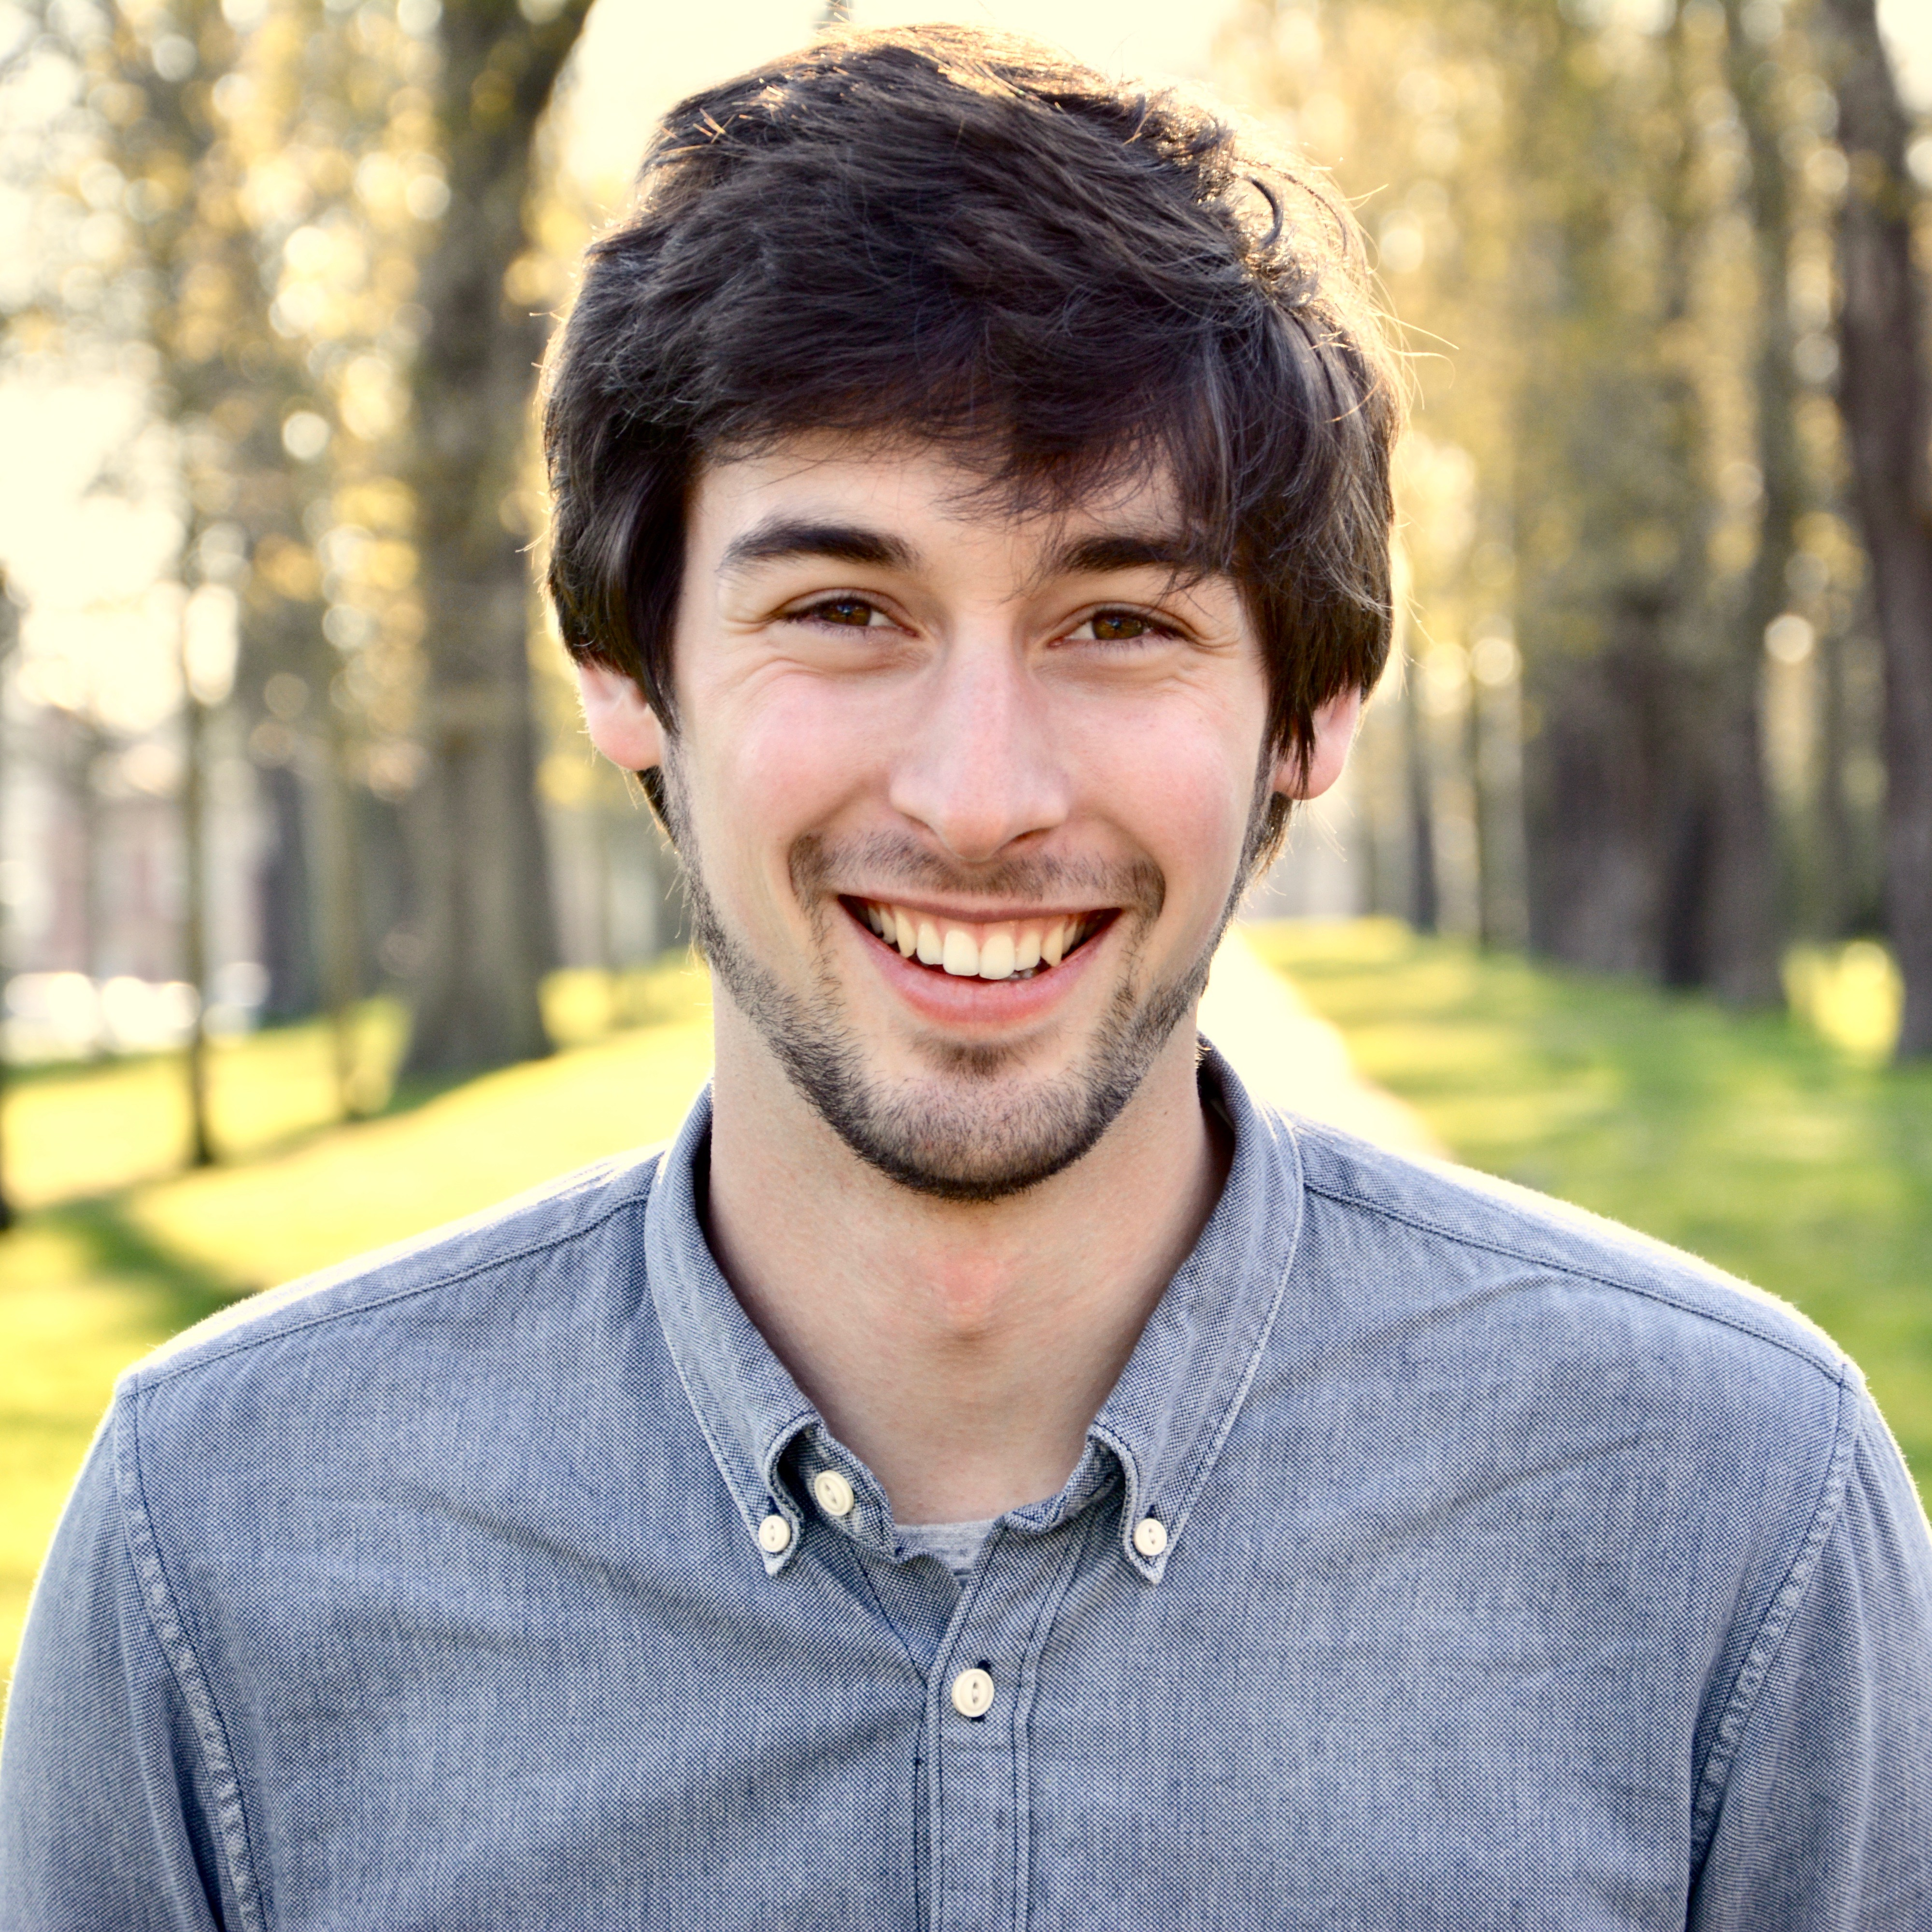
\includegraphics[width=1.2\linewidth]{figs/DSC_2812.jpg}
  \end{minipage}
  %&
  \begin{minipage}{.74\textwidth}
    \begin{center}
      % Title 
      \huge \textbf{scpdata: a data package for single-cell proteomics} \\
      \vspace{0.4cm}
      % Authors
      \Large \textbf{Christophe Vanderaa, Laurent Gatto} \\
      % Affiliation
      \Large \textit{Computational biology and bioinformatics lab, de Duve Institute, UCLouvain } \\
      % email
      \vspace{0.4cm}
      \normalsize christophe.vanderaa@uclouvain.be \\
    \end{center}
  \end{minipage}
  %&
  \begin{minipage}{3.7cm}
      \includegraphics[width=0.7\linewidth, right]{figs/fnrs.png} \\
      \vspace{0.5cm}
      \includegraphics[width=1.1\linewidth, right]{figs/ucl.png}
  \end{minipage}
}
\end{center}


% ---------------------------------------------------------------------------

\setlength{\columnsep}{1cm}
\begin{multicols}{2}

\noindent
\fcolorbox{yellow}{yellow}{
  \begin{minipage}[t]{\linewidth}
    \vspace{.05cm}
      \vspace{.1cm}
      \section*{\huge Summary}
      \Large Recent advances in sample preparation, processing and mass spectrometry (MS) have allowed the emergence of MS-based single-cell proteomics (SCP). However, bioinformatics tools to process and analyze these new types of data are still missing. In order to boost the development and the benchmarking of SCP methodologies, we are developing the scpdata experiment package. The package will distribute published and curated SCP data sets in standardized Bioconductor format. 
    
  \end{minipage}
}

% ---------------------------------------------------------------------------

\section*{Introduction}

There are two main types of MS-SCP data:

\begin{itemize}
  \item Label-free proteomics: the nanoPOTS technology developed by Zhu and colleagues (@Zhu2018-bf) analyzes one sample/cell per MS run. Although the throughput is low (~10 samples/day), it allows for an accurate peptide quantification. 
  \item TMT-based proteomics: the SCoPE pipeline developed by the Slavov Lab (@Budnik2018-qh) combines different samples/cells in a single MS run using tandem-mass tags (TMT) labeling. It increases the throughput and the identification rate, but reduces the quantification accuracy.
\end{itemize}

Data will be available for both techniques. This allows an informed choice for which statistical method to use for a given technique.


% ---------------------------------------------------------------------------

\vspace{.2cm}

\noindent
\colorbox{marronrp3}{
  \begin{minipage}[t]{.96\linewidth}
    \Large
    \begin{align*}
      \frac{d}{dt} c_j
      & = &&  \frac{1}{2} \sum_{k=1}^{j-1} a_{k,j-k}  c_k c_{j-k}
      &  \text{Coagulation gain}\\
      && - &\sum_{k=1}^{\infty} a_{jk} c_j c_k
      &   \text{Coagulation loss}\\
      && + &\sum_{k=j+1}^{\infty} b_{j,k-j} c_k
      &   \text{Fragmentation gain}\\
      && - &\frac{1}{2} \sum_{k=1}^{j-1} b_{k,j-k} c_j
      & \text{Fragmentation loss}
    \end{align*}
    \vspace{.02cm}
  \end{minipage}
}
\vspace{.4cm}

{\textcolor{rojo}{The generalized Becker-Döring system is the special
    case where $a_{jk}$ and $b_{jk}$ are zero whenever $\min\{j,k\} >
    N$ for some $N$. For $N=1$ the system is the Becker-Döring
    system.}  }

\section*{Asymptotic Behavior}

The study of the long-time behavior of solutions to these equations is
expected to be a model of physical processes such as phase transition.
Under certain general conditions which include a detailed balance we
can ensure the existence of equilibrium states. In these conditions,
there is a critical mass $\rho_s \in ]0,\infty[$ such that any
solution that initially has mass $\rho_0 \leq \rho_s$ will converge
for large times, in a certain strong sense, to an equilibrium solution
with mass $\rho_0$. On the other hand, any solution with mass above
$\rho_s$ converges (in a weak sense) to the only equilibrium with mass
$\rho_s$; this weak convergence can then be interpreted as a phase
transition in the physical process modelled by the equation.

Convergence in this weak sense means that a fixed part of the total
mass of particles is found to be forming larger and larger clusters as
time passes and the mean size of clusters goes to infinity. The
physical interpretation of this, depending on the context, can be a
change of phase or the apparition of crystals, for example.

\noindent
\begin{center}
  \noindent
  \colorbox{marronrp3}{
    \begin{minipage}[t]{.96\linewidth}
      \begin{align*}
        & \text{\Large Below critical mass}
        &\to \quad
        &\begin{cases}
          \text{ \Large Trend to equilibrium }\\
          \text{ \Large Strong convergence }
        \end{cases}
        &
        \\
        &\text{\Large Over critical mass }
        &\to \quad
        &\begin{cases}
          \text{ \Large Large clusters created}\\
          \text{\Large Weak convergence }
        \end{cases}
        &
      \end{align*}
    \end{minipage}
  }
\end{center}

\begin{center}  

\vspace{.5cm}

\Large
\begin{tabular}[t]{c|c}
  \multicolumn{2}{c}{\huge \textbf{Previous results}}
  \vspace{.3cm}
  \\
  Becker-Döring& Ball, Carr, Penrose\\
  system       & \cite{BCP86,BC88} (1986-88)\\
  \hline
  Generalized Becker-Döring &Carr, da Costa\\
  (rapidly decaying initial data) &\cite{CdC94} (1994)\\
  \hline
  Generalized Becker-Döring & da Costa \\
  (small initial data) & \cite{dC98} (1998)
\end{tabular}
\end{center}


% ---------------------------------------------------------------------------
  
\section*{Sketch of the proof}

Our proof is a generalization of a method used in unpublished notes by
Ph. Lauren\c{c}ot and S. Mischler \cite{LM}, inspired by the proof of
uniqueness of solutions to the Becker-D\"oring equation in
\cite{LM02e}.

It is known that, under common assumptions, \emph{there is always} at
least weak convergence to a certain equilibrium state;
\textcolor{rojo}{the problem reduces to show that for an initial
  density under the critical one solutions converge \emph{strongly} to
  the equilibrium \emph{with the same density}}. To prove this, it is
enough to show that the tails of the solutions are small enough, so
that strong convergence holds. The following estimate, roughly stated
here, is the key of our proof:

\noindent
\colorbox{marronrp3}{
  \begin{minipage}[t]{.96\linewidth}
    \vspace{.2cm}
    \centerline{\huge \textbf{Main estimate}}
    \vspace{.05cm}

    \Large
    If $c = \{c_j\}_{j \geq 1}$ is a solution to the generalized
    Becker-Döring equations with density below the critical one, then
    there is some sequence $r_i$ (which tends to zero as $i \to
    \infty$) such that the tails of the solution have mass below
    $r_i$; this is,
    \begin{equation*}
      \sum_{k=i}^\infty k c_k(t) \leq r_i
    \end{equation*}
    for all times $t$ after some time $t_0$.
    \\\hspace{.05cm}
  \end{minipage}
}

\vspace{.5cm}

The proof of this consists mainly of an estimate obtained by
differentiating the quantity $H_i := (G_i-r_i)_+$ (the positive part
of $G_i - r_i$), proving with a differential inequality that it must
remain zero for all times starting from a certain $t_0$.
% ---------------------------------------------------------------------------
%
\small
\begin{thebibliography}{}

\bibitem{BCP86} J. M. Ball, J. Carr, O. Penrose, \emph{The
    Becker-D\"oring cluster equations: basic properties and asymptotic
    behaviour of solutions}, Comm. Math. Phys. 104, 657--692 (1986)

\bibitem{BC88} J. M. Ball, J. Carr, \emph{Asymptotic behaviour of
    solutions to the Becker-D\"oring equations for arbitrary initial
    data}, Proc. Roy. Soc. Edinburgh Sect. A, 108, 109-116 (1988)
  
\bibitem{C04} J. A. Cañizo, \emph{Asymptotic behavior of solutions to
    the generalized Becker-Döring equations for general initial data},
  preprint.
  
\bibitem{CdC94} J. Carr, F. P. da Costa, \emph{Asymptotic behaviour of
    solutions to the coagulation-fragmentation equations. II. Weak
    fragmentation}, J. Stat. Phys. 77, 89--123 (1994)

\bibitem{dC98} F. P. da Costa, \emph{Asymptotic behaviour of low
    density solutions to the generalized Becker-D\"oring equations},
  NoDEA Nonlinear Differential Equations Appl. 5, 23--37, (1998)
  
\bibitem{LM} Ph. Lauren\c{c}ot, S. Mischler, \emph{Notes on the
    Becker-D\"oring equation}, personal communication.

\bibitem{LM02e} Ph. Lauren{\c{c}}ot, S. Mischler, \emph{From the
    {B}ecker-{D}\"oring to the {L}ifshitz-{S}lyozov-{W}agner
    equations}, J. Statist. Phys. 106, 5-6, pages 957--991 (2002).

\end{thebibliography}


\end{multicols}

\end{document}